\documentclass[12pt]{article}
%\usepackage{times}
\usepackage{cite}
\usepackage{graphicx}
\usepackage{url}
\setlength{\parskip}{1em}
\setlength{\parindent}{0em}
%this is a comment
\title{CS 361 \\ User Stories and Set-up Assignment (USSA): \\ Digital Ghostwriter}
\author{Thomas Hollenberg (hollenbt), Zachary Thomas (thomasza),\\ Amar Raad (raadv), Jared Tence (tencej), \\  Zech DeCleene (decleenz)}
\date{February 25th, 2018}

\begin{document}
\maketitle
\newpage
\tableofcontents

\newpage

\section{User Stories}

\textbf{Comedy genre}\newline
Should have a selectable comedy genre in the genre and writing menus.
Should generate stories with comedy model.

\textbf{Drama genre}\newline
Should have a selectable drama genre in the genre and writing menus.
Should generate stories with drama genre.

\textbf{Horror genre}\newline
Should have a selectable horror genre in the genre and writing menus.
Should generate stories with horror genre.

\textbf{Science fiction genre}\newline
Should have a selectable science fiction genre in the genre and writing menus.
Should generate stories with science fiction genre.

\textbf{Mystery genre}\newline
Should have a selectable mystery genre in the genre and writing menus.
Should generate stories with the mystery genre.

\textbf{User created genre}\newline
User should be able to create a new genre.
The genre will be selectable in the genre and writing menus.
Should generate stories with the new genre.

\textbf{View genres}\newline
Should be able to view all default genres.
Should be able to view all created genres.

\textbf{Delete genre}\newline
Users should be able to delete default genres.
Users should be able to delete created genres.

\textbf{Delete authors}\newline
Users should be able to delete authors from a genre.

\textbf{Add authors}\newline
Should be able to add an author to a genre.

\textbf{View authors}\newline
Should be able to view all authors in a genre.

\textbf{Selectable word count}\newline
When generating a story users should be able to select a word count.

\textbf{Generate story as text document}\newline
When generating a story, the new story is output as a text document on the computer.

\textbf{Naming story}\newline
When generating a story users should be able to select a name for the file that is created.

\textbf{Exit Program}\newline
Should be able to close program.

\textbf{Previous Page}\newline
Should be able to go back to a previous page.

\textbf{Grammar and Syntax Check}\newline
After creating document, it is checked for Syntax errors.
After creating document, it is checked for Grammar errors.
 
\textbf{Set output destination}\newline
User should be able to change the location that the output file goes to.

\textbf{Generate multiple stories at once}\newline
User should be able to select how many stories they want digital ghostwriter to write, so they can output multiple stories at once.

\textbf{Copy genre}\newline
Users should be able to copy a genre to a new name so that they may make changes without deleting the original.

\newpage

\section{Corresponding Tasks}

\textbf{Comedy genre}\newline
Due: Two weeks from now.
\newline
Tasks: 
\newline
1. Create genre model.
\newline
2. Display genre in genre and write menus.
\newline
3. Enable usage of model to create stories.
\newline
Prerequisites: None.
\newline
Effort estimate: 2 units. 

\textbf{Drama genre}\newline
Due: Two weeks from now.
\newline
Tasks: 
\newline
1. Create genre model.
\newline
2. Display genre in genre and write menus.
\newline
3. Enable usage of model to create stories.
\newline
Prerequisites: None.
\newline
Effort estimate: 2 units. 

\textbf{Horror genre}\newline
Due: Next week.
\newline
Tasks: 
\newline
1. Create genre model.
\newline
2. Display genre in genre and write menus.
\newline
3. Enable usage of model to create stories.
\newline
Prerequisites: None.
\newline
Effort estimate: 2 units. 

\textbf{Science fiction genre}\newline
Due: Two weeks from now.
\newline
Tasks: 
\newline
1. Create genre model.
\newline
2. Display genre in genre and write menus.
\newline
3. Enable usage of model to create stories.
\newline
Prerequisites: None.
\newline
Effort estimate: 2 units. 

\textbf{Mystery genre}\newline
Due: Two weeks from now.
\newline
Tasks: 
\newline
1. Create genre model.
\newline
2. Display genre in genre and write menus.
\newline
3. Enable usage of model to create stories.
\newline
Prerequisites: None.
\newline
Effort estimate: 2 units. 

\textbf{User created genre}\newline
Due: Three weeks from now.
\newline
Tasks: 
\newline
1. Create interface for new genre creation.
\newline
2. Dynamically generate new model with user selected name.
\newline
3. Dynamically display genre in genre and write menus.
\newline
4. Enable usage of model to create stories.
\newline
Prerequisites:
\newline
Genre must be viewable before this feature can be implemented.
\newline
Effort estimate: 15 units. 

\textbf{Delete genre}\newline
Due: Three weeks from now.
\newline
Tasks:
\newline
1. Remove genre folder from file system, as well as the contained model and training material.
\newline
2. Remove genre from GUI display, and destroy genre object in memory.
\newline
Prerequisites: 
\newline
Genre must be viewable before this feature can be implemented.
\newline
Genre to be removed is in the genre list.
\newline
Effort estimate: 2 units.

\textbf{View genres}\newline
Due: Next week.
\newline
Tasks: 
\newline
1. Create page to display genres.
\newline
2. Display all genres on the page.
\newline
Prerequisites: Any genre.
\newline
Effort estimate: 5 units.

\textbf{Delete authors}\newline
Due: Three weeks from now.
\newline
Tasks: 
\newline
1. Remove author from author list, and retrain genre. 
\newline
2. Remove author from GUI.
\newline
Prerequisites: 
\newline
Genre must be viewable before this feature can be implemented.
\newline
Authors must be viewable before this feature can be implemented.
\newline
Author to be removed is in the author list.
\newline
Effort estimate: 4 units.

\textbf{Add authors}\newline
Due: Three weeks from now.
\newline
Tasks: 
\newline
1. Design interface to allow users to add authors to genre.
\newline
2. Update genre model based on new authors input.
\newline
Prerequisites:
\newline
Genre must be viewable before this feature can be implemented.
\newline
Authors must be viewable before this feature can be implemented.
\newline
Effort estimate: 10 units. 

\textbf{View authors}\newline
Due: Next week.
\newline
Tasks: 
\newline
1. Make genres function as buttons, when clicked on brings you to new menu.
\newline
2. In new menu display all current author files by name.
\newline
Prerequisites:
\newline
Genre must be viewable before this feature can be implemented.
\newline
Any author.
\newline
Effort estimate: 3 unit. 

\textbf{Selectable word count}\newline
Due: Three weeks from now.
\newline
Tasks:
\newline
1. Create text entry field that allows user to indicate desired word count.
\newline
2. Pass the value of this field to the sample.py program upon submission so that the output contains the desired word count.
\newline
Prerequisites: 
\newline
Generate story as text document must be implemented first.
\newline
Any genre.
\newline
Effort estimate: 4 units.

\textbf{Generate story as text document}\newline
Due: Two weeks from now.
\newline
Tasks:
\newline
1. Setup user selections (otherwise use defaults).
\newline
2. Run genre model through tensorflow to create story.
\newline
3. Output tensorflow to text document in "stories" directory.
Prerequisites: Any genre.
\newline
Genre must be viewable before this feature can be implemented.
\newline
Effort estimate: 10 units.

\textbf{Naming story}\newline
Due: Two weeks from now.
\newline
Tasks:
\newline
1. Create pop up that allows user to enter name of story.
\newline
2. Names the document created by tensorflow to that name.
\newline
Prerequisites:
\newline
Generate story as text document must be implemented first.
\newline
Effort estimate: 2 units.

\textbf{Exit Program}\newline
Due: Next week.
\newline
Tasks: 
\newline
1. Create task bar button.
\newline
2. Make button terminates program.
\newline
Prerequisites: None.
\newline
Effort estimate: 1 unit. 

\textbf{Previous Page}\newline
Due: Next week.
\newline
Tasks: 
\newline
1. Create task bar button.
\newline
2. Make button return to previous menu.
\newline
Prerequisites: None.
\newline
Effort estimate: 2 units. 

\textbf{Grammar and Syntax Check}\newline
 Due: Three weeks from now.
\newline
Tasks: 
\newline
1. Define grammar/syntax rules.
\newline
2. Implement scanner/parser to enforce rules.
\newline
Prerequisites: Generate text output.
\newline
Effort estimate: 5 units. 

\textbf{Set output destination}\newline
Due: Two weeks from now.
\newline
Tasks: 
\newline
1. Create new GUI page with text entry field to allow user to change output path.
\newline
2. Update local output path variable so that generated text is saved in the desired location.
\newline
Prerequisites: None.
\newline
Effort estimate: 2 unit. 

\textbf{Generate multiple stories at once}\newline
Due: Three weeks from now.
\newline
Tasks:
\newline
1. Create option for making multiple stories at once.
\newline
2. Output multiple stories into same directory.
\newline
Prerequisites: Any genre.
\newline
Effort estimate: 5 units.

\textbf{Copy genre}\newline
Due: Three weeks from now.
\newline
Tasks:
\newline
1. Copy genre folder, as well as the contained model and training material.
\newline
2. Paste folder with a new name, and rename the model file within.
\newline
3. Add copy to GUI display and create genre object in memory.
\newline
Prerequisites: Any genre.
\newline
Effort estimate: 2 units.

\newpage

\section{UML Sequence Diagram/Spike}

\begin{figure}[ht]
  \centering
    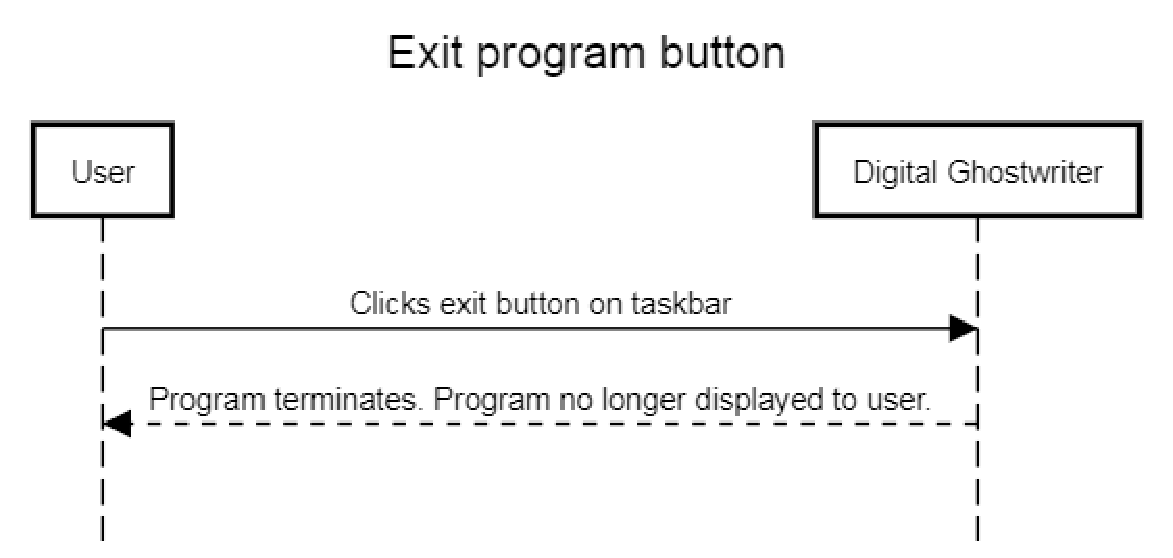
\includegraphics[scale=0.7]{Exit.eps}
\end{figure}

\begin{figure}[ht]
  \centering
    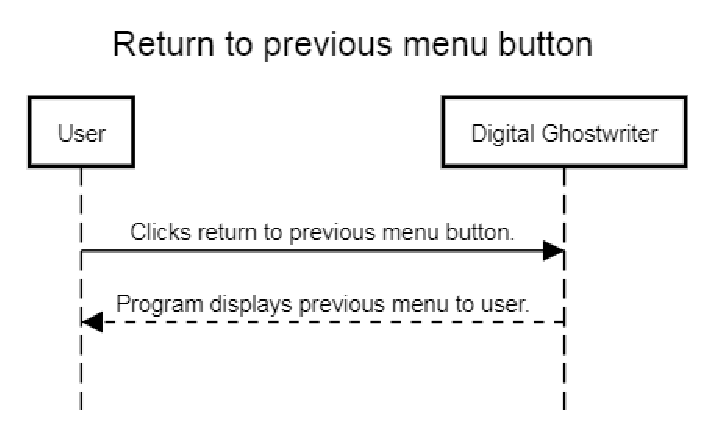
\includegraphics[scale=1]{Return.eps}
\end{figure}

\newpage

\begin{figure}[ht]
  \centering
    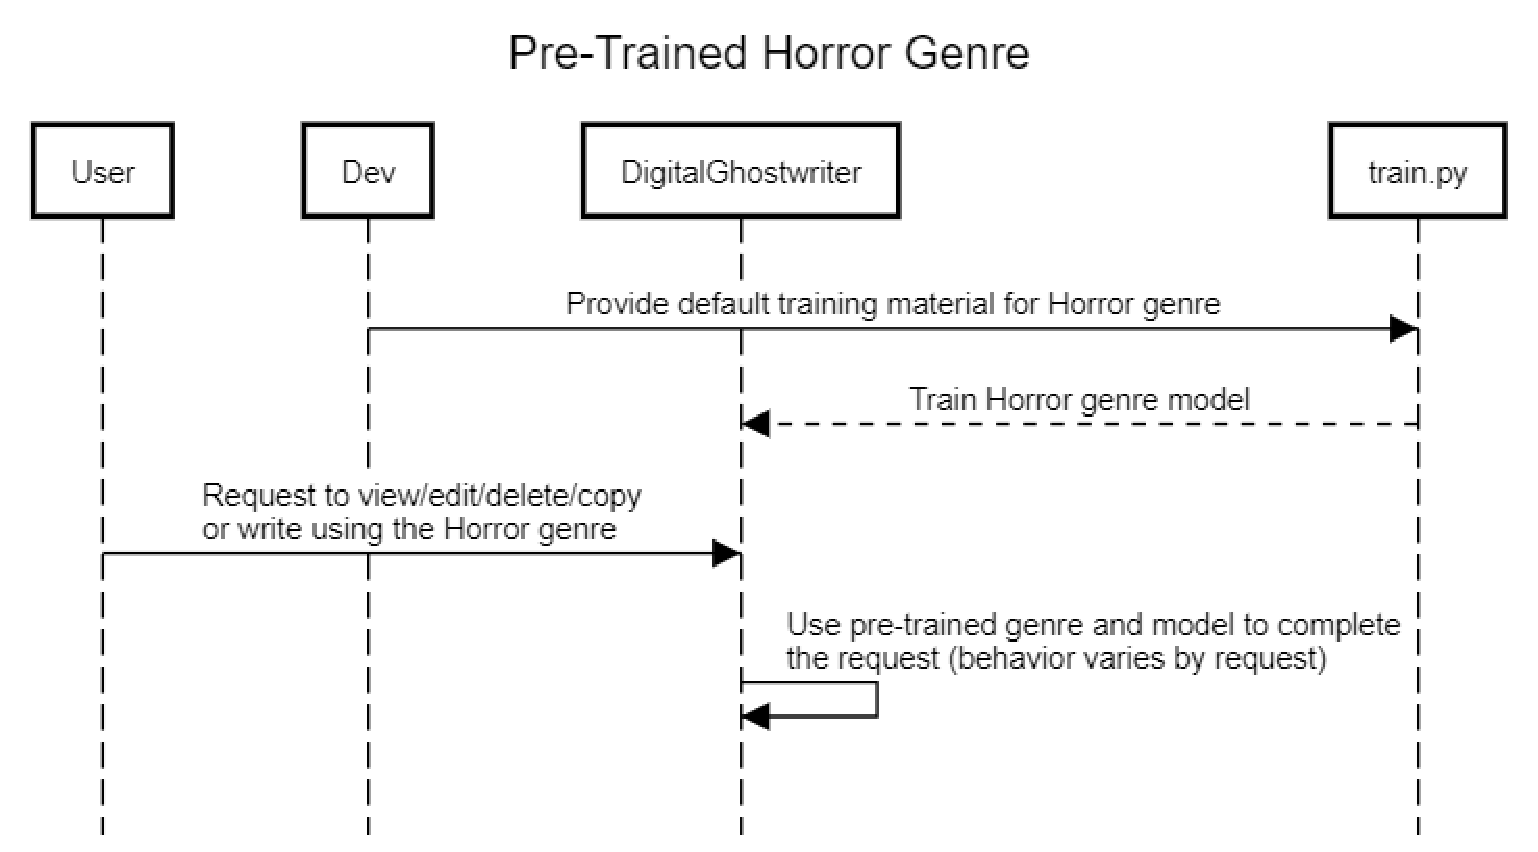
\includegraphics[scale=0.6]{Horror.eps}
\end{figure}

\newpage 

\begin{figure}[ht]
  \centering
    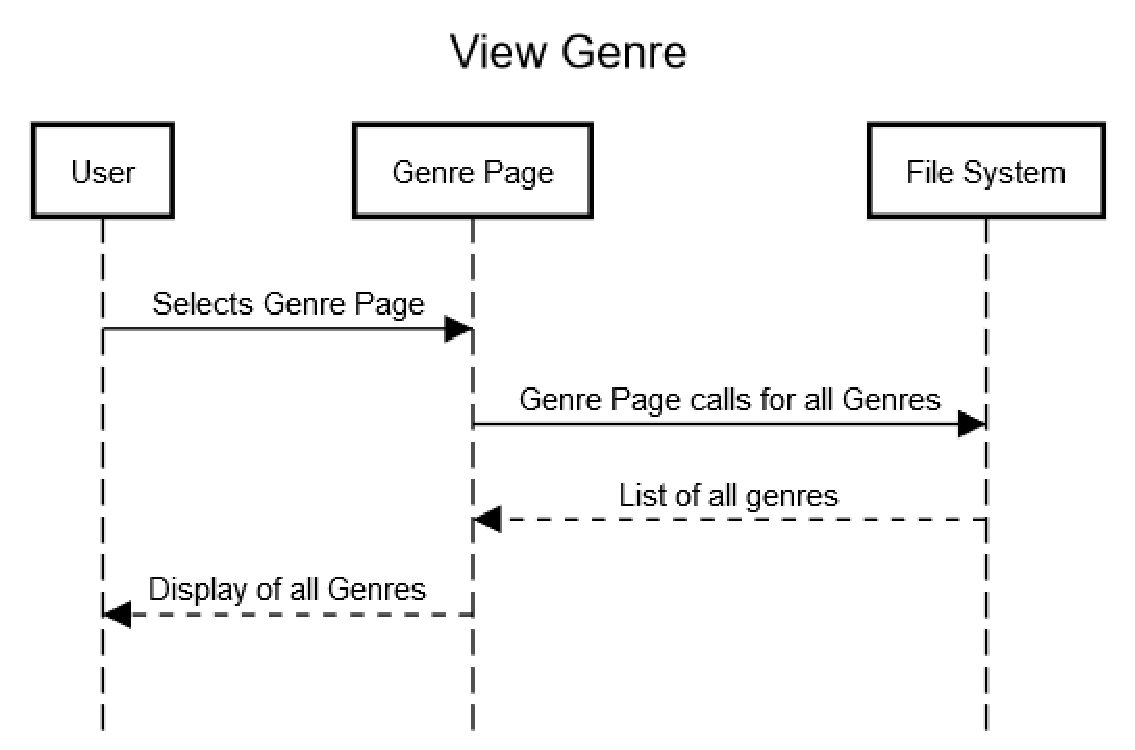
\includegraphics[scale=0.7]{Genre.eps}
\end{figure}

\begin{figure}[ht]
  \centering
    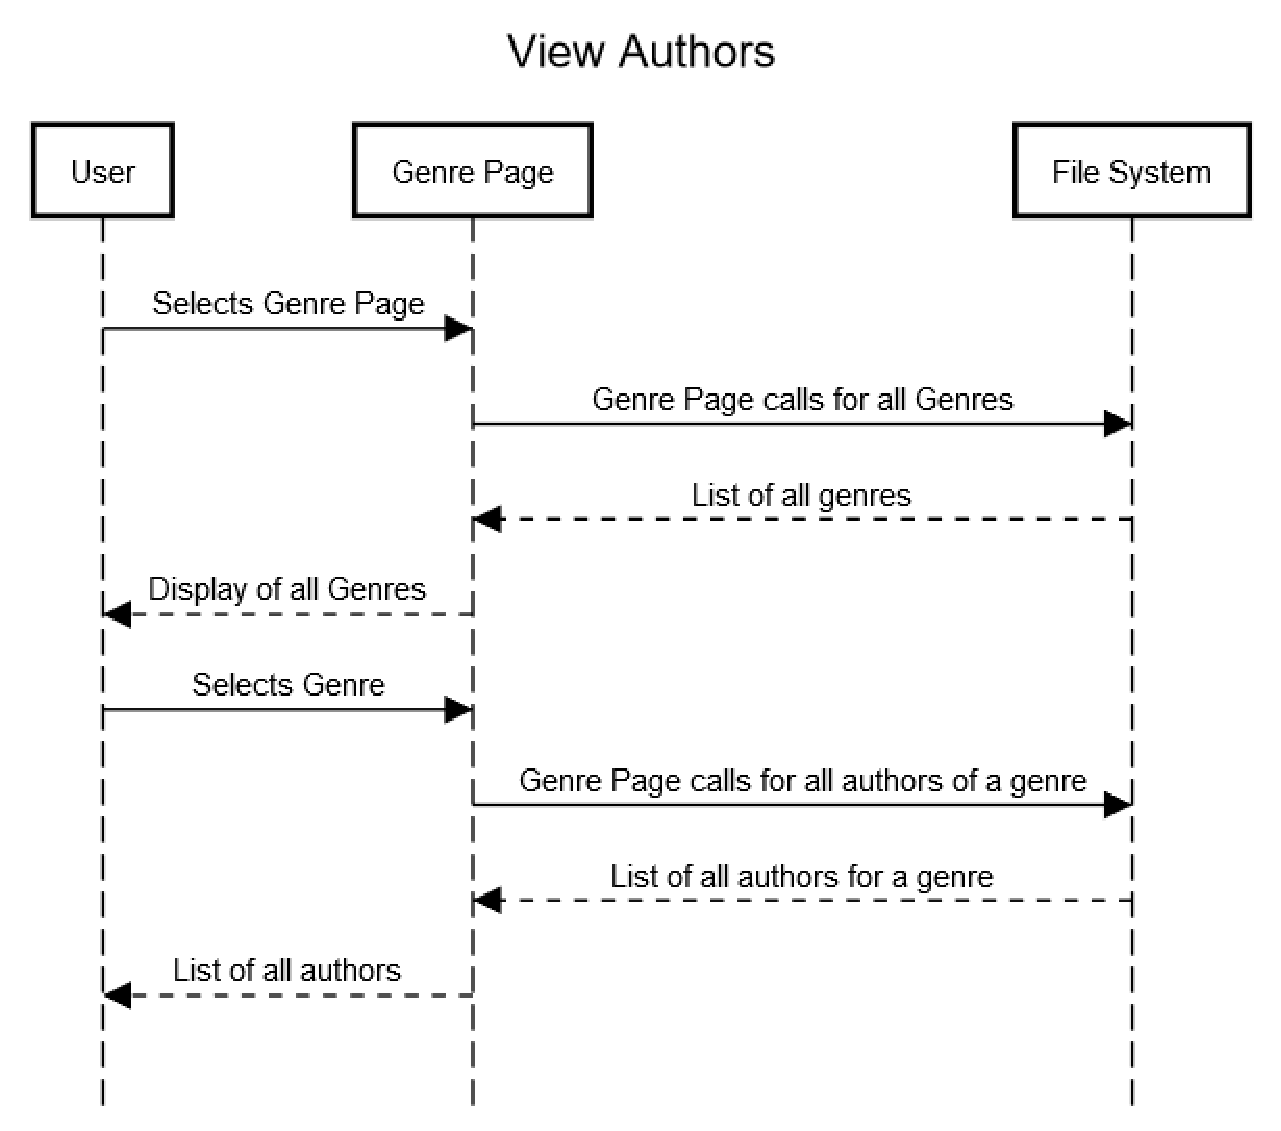
\includegraphics[scale=0.7]{Author.eps}
\end{figure}

\newpage

\section{The Stories due Next Week }

Teams will be randomly cycled in pairs to work on sections of the project.

Monday we will implement \textbf{Exit Program} and \textbf{Previous Page} user stories.

Tuesday we will be having a group meeting at JOHN on campus to start tackling the larger user stories and plan further.

Wednesday we will complete the \textbf{Horror genre}
and \textbf{View genres} user stories.

Thursday we will have the whole team finish the \textbf{View authors} user story.

\section{Meeting Report }

\subsection{This week's progress:}
Made further progress on implementation of Digital Ghostwriter, added in word-rnn Tensorflow that now interfaces with GUI.

\subsection{Goals for next week:}
Tuesday meeting at 3pm at JOHN to discuss and collaborate on our Digital Ghostwriter implementation. Learn and implement canvas on our GUI. Complete exit program, previous page, horror genre, view genres and view authors.

\subsection{Contribution of team members:}
All team members gave feedback and worked on our assignment.

\subsection{Were customers able to meet with the team:}
Yes. Team including customers met to complete assignment and talk about improvements on the GUI.

\end{document}
